\chapter{Probability in Practice: Stochastic Estimators}

The accuracy of deterministic estimators will always be limited by
the flexibility of the approximating distribution to match the geometry 
of the typical set of the target distribution.  The only way to overcome
this restriction is to quantify the typical set of the target distribution
directly.  Unfortunately, this presents problems of its own as in practice 
we don't know where to find the typical set in the expansive sample space.  
Because exhaustive search of the sample space is far too expensive
we need a more targeted procedure for finding and then exploring 
the typical set.

By construction an infinite number of samples from the target distribution 
quantifies the typical set, and hence the samples themselves provide
a natural way to identify the typical set (Figure \ref{fig:samples}).  The
utility of samples, however, depends both on how precisely we can 
quantify the typical set using only a finite number of samples and how
well we can generate samples in the first place.

\emph{Stochastic estimators} use samples, either from the target probability
distribution or auxiliary probability distributions, to construct estimators 
of the expectation with respect to the target distribution.  Exactly how these
samples are generated leads to estimators with substantially different 
behaviors.

\subsection{Monte Carlo Estimators}

Monte Carlo estimators use a finite sequence of exact samples from
the target distribution to estimate expectations.  Given a sequence
of exact samples $\left\{ \theta_{1}, \ldots, \theta_{N} \right\}$ we can
construct a  \emph{Monte Carlo estimator} of the expectation of 
\emph{any} function $f : \Theta \rightarrow \RR$ as
%
\begin{equation*}
\hat{f}^{\mathrm{MC}}_{N} \equiv
\frac{1}{N} \sum_{n = 1}^{N} f \! \left( \theta_{n} \right).
\end{equation*}

By construction these Monte Carlo estimators recover the exact
expectation asymptotically,
%
\begin{equation*}
\lim_{N \rightarrow \infty} \hat{f}^{\mathrm{MC}}_{N}
=
\EE_{\PP} [ f ],
\end{equation*}
%
but they are also accurate even when the sequence is finite.
Provided that the samples are exact, Monte Carlo estimators 
follow a Central Limit Theorem -- for sufficiently large $N$ the 
estimators themselves follow a distribution given by a Gaussian 
density,
%
\begin{equation*}
\hat{f}_{N} \sim 
\mathcal{N} \! \left( \EE_{\PP} [ f ],
\mathrm{MCSE} \right),
\end{equation*}
%
where the \emph{Monte Carlo Standard Error} is defined as
%
\begin{equation*}
\mathrm{MCSE } \equiv \sqrt{ \frac{ \mathrm{Var} [ f ] }{N} }.
\end{equation*}
%
Consequently Monte Carlo estimators are unbiased with respect
to all of the possible sequences we could have generated, and 
their precision improves as we generate more and more samples.
Moreover, functions with high variance are more challenging to
estimate than those with low variance.

In practice we use another Monte Carlo estimator to approximate the
variance $\mathrm{Var} [ f ] $, and hence the Monte Carlo Standard
Error itself.  The error of this approximation is
%
\begin{equation*}
\sqrt{\mathrm{Var} [ \, \mathrm{Var} [ f ]  \, ] / N^{2} },
\end{equation*}
which is typically negligible compared to the Monte Carlo Standard Error 
of $f$.  Monte Carlo estimators, then, are distinct from deterministic 
approximations in that they naturally come equipped with a procedure 
for at least estimating their error.

Of course all of these benefits of Monte Carlo estimators are dependent 
on our ability to generate exact samples from the target probability 
distribution.  Unfortunately, generating exact samples is infeasible for all 
but the simplest probability distributions, and we are once again frustrated 
by our ignorance of the typical set.  In order to proceed we need to 
approximate exact samples themselves.

\subsection{Importance Sampling Estimators}

Although we typically can't generate exact samples from the target 
distribution, often we can generate exact samples from an 
\emph{auxiliary} probability distribution, $\mathbb{G}$,
%
\begin{equation*}
\left\{ \vartheta_{1}, \ldots, \vartheta_{N} \right\} \sim \mathbb{G}.
\end{equation*}
%
\emph{Importance sampling estimators} use these auxiliary samples 
corrected with \emph{importance weights}, $w \! \left( \vartheta \right)$,  
%
\begin{equation*}
\EE_{\PP} [ f ] \approx 
\hat{f}^{\mathrm{IS}}_{N} = 
\frac{1}{N} \sum_{n = 1}^{N} 
w \! \left( \vartheta_{n} \right) f \! \left( \vartheta_{n} \right)
\end{equation*}
%
If $p$ and $g$ are the probability density functions corresponding to
the target distribution and auxiliary distribution, respectively, then the 
importance weights are given by
%
\begin{equation*}
w \! \left( \vartheta_{n} \right) =
\frac{ p \! \left( \vartheta_{n} \right) }
{ g \! \left( \theta_{n} \right) }.
\end{equation*}
%
Although they are constructed from probability density functions, 
importance weights, and hence importance sampling estimators,
are invariant to the choice of sample space.  When we map to
an equivalent sample space, the resulting Jacobian is the same
in both the numerator and denominator and consequently cancels 
when evaluating the weights themselves.

Given certain regularity conditions, importance sampling estimators 
also satisfy a Central Limit Theorem
%
\begin{equation*}
\hat{f}_{N}^{\mathrm{IS}} \sim 
\mathcal{N} \! \left( \EE_{\PP} [ f ],
\mathrm{ISSE} \right),
\end{equation*}
%
The \emph{Importance Sampling Standard Error} is given by
%
\begin{equation*}
\mathrm{ISSE} \equiv \sqrt{ \frac{ \mathrm{Var} [ f ] }{\mathrm{ESS} } },
\end{equation*}
%
with the \emph{effective sample size} defined as
%
\begin{equation*}
\mathrm{ESS} = 
N 
\frac{ \left( \sum_{n = 1}^{N} w \! \left( \vartheta_{n} \right) \right)^{2} }
{ \sum_{n = 1}^{N} w \! \left( \vartheta_{n} \right)^{2} }.
\end{equation*}
%
Comparing this to the Monte Carlo Central Limit Theorem we can
see that the effective sample size quantifies how many exact
samples would have yielded the same estimator precision,
hence the effective sample size can be interpreted as the
effective number of exact samples ``contained'' in the auxiliary
samples.

The challenge with constructing a useful importance sampler is
finding an auxiliary distribution that is not too different from the
target distribution.  Although importance sampling estimators are 
unbiased, their variance can be so large as to be impractical when 
the auxiliary distribution deviates too strongly from the target distribution 
and the weights are large.  In fact, when the auxiliary distribution has 
lighter tails than the target distribution these estimators can 
easily have infinitely large variance: not only does this make 
the estimators themselves useless, it also makes estimates of 
the variance and hence any quantification of the estimator error 
useless.

Selecting an auxiliary distribution that yields accurate importance
sampling estimators, however, is challenging without knowing
the structure of the typical set a priori.  Ultimately, importance
sampling is most useful as a means to correct a distribution that 
is already known to be a good approximation to the target
distribution.

\subsection{Markov Chain Monte Carlo Estimators}

Another strategy for approximating the Monte Carlo procedure
is to generate samples from the target distribution but relax
the requirement that they be exact.  Fortunately, correlated 
samples are readily given by \emph{Markov chains}.

A Markov chain is a stochastic processes generated not by a
static probability distribution but by a probability distribution 
that depends on the last state in the sequence.  In other words, 
each state in the sequence is sampled from a conditional 
probability distribution known as a \emph{Markov transition 
kernel}, $\mathbb{T}$, 
%
\begin{align*}
\mathbb{T}
&: \EV{\Theta} \times \Theta \rightarrow \left[0, 1 \right] \\
&\quad \left( E, \theta \right) \;\; \mapsto 
\mathbb{T} \! \left[ E \mid \theta \right].
\end{align*}
%
When the Markov transition operator preserves the target
distribution,
%
\begin{equation*}
\PP \! \left[ E \right]
=
\mathbb{E}_{\PP} \! 
\left[  \mathbb{T} \! \left[ E \mid \theta \right] \right]
\end{equation*}
%
or, with respect to probability density functions,
%
\begin{equation*}
p \! \left( \theta \right)
=
\int_{\Theta} t \! \left( \theta' \mid \theta \right) 
\pi \! \left( \theta' \right) \dd \theta',
\end{equation*}
%
then the Markov chain asymptotically recovers expectations
with \emph{Markov chain Monte Carlo estimators},
%
\begin{equation*}
\lim_{N \rightarrow \infty} 
\hat{f}^{\mathrm{MCMC}}_{N}
\equiv
\lim_{N \rightarrow \infty} 
\frac{1}{N} \sum_{n = 1}^{N} f \! \left( \theta_{n} \right)
=
\mathbb{E}_{\PP} \! \left[ f \right],
\end{equation*}
%
and we can interpret the Markov chain itself as a sequence
of correlated samples from the target distribution.

More intuitively, the Markov transition kernel quantifies
the variability in each step of the Markov chain.  When the
transition preserves the target distribution, then it 
concentrates closer to the typical set than away from it --
it is literally attracted to the typical set.  Consequently, the
Markov chain will eventually find and then explore the
typical set no matter where we start in the sample space,
and the Markov chain Monte Carlo estimators will converge
to the true expectations.
 
The important caveat here is that the Markov chain is 
guaranteed to find and fully explore the typical set only 
asymptotically.  In practice, however, it is the only the finite time 
performance of Markov chains that matters and, unfortunately, the 
finite time behavior of Markov chain Monte Carlo is much more
subtle than its exact predecessor.

In this section we discuss how Markov chain Monte Carlo
behaves under ideal conditions, how it behaves under
less-than-ideal conditions, and how to effectively run
the algorithm in practice to be robust to the latter.

\subsubsection{Markov Chain Monte Carlo Under Ideal Conditions}

Under ideal conditions, Markov chains explore the target
distribution in three distinct phases.  In the first phase the
Markov chain converges towards the typical set from its
initial position and Markov chain Monte Carlo estimators
are highly biased (Figure \ref{fig:ideal_mcmc}a).  The
second phase begins once the Markov chain finds the
typical set and persists through the first sojourn across
the typical set.  This initial exploration is extremely effective
and the accuracy of Markov chain Monte Carlo estimators
rapidly improves as the bias from the initial samples is
eliminated (Figure \ref{fig:ideal_mcmc}b).  The third phase 
consists of all subsequent exploration where the the Markov 
chain refines its exploration of the typical set and the precision 
of the Markov chain Monte Carlo estimators improves, albeit 
at a slower rate (Figure \ref{fig:ideal_mcmc}c).

\begin{figure*}
\centering
\subfigure[]{
\begin{tikzpicture}[scale=0.25, thick]
  \draw[-,color=white] (-12, 0) to (12, 0);
  
  \begin{scope}
  \clip (-12, -10) rectangle (12, 10);
  
  \foreach \i in {0, 0.05,..., 1} {
    \draw[line width={30 * \i}, opacity={exp(-8 * \i)}, dark] 
      (-10, 0) .. controls (-10, 15) and (-5, 5) .. (0, 5)
      .. controls (5, 5) and (10, 8) .. (10, 0)
      .. controls (10, -8) and (5, -3) .. (0, -3)
      .. controls (-5, -3) and (-10, -5) .. (-10, 0);
  }

  %\fill[color=dark] (-11, -8) circle (7pt);  
  %\fill[color=light] (-11, -8) circle (5pt);
  
  \fill[color=dark] (-10, -6.5) circle (7pt);  
  \fill[color=light] (-10, -6.5) circle (5pt);
  
  \fill[color=dark] (-9, -6.75) circle (7pt);  
  \fill[color=light] (-9, -6.75) circle (5pt);
  
  \fill[color=dark] (-8.25, -5) circle (7pt);  
  \fill[color=light] (-8.25, -5) circle (5pt);
  
  \fill[color=dark] (-7.5, -4) circle (7pt);  
  \fill[color=light] (-7.5, -4) circle (5pt);
  
  \fill[color=dark] (-7, -3.5) circle (7pt);  
  \fill[color=light] (-7, -3.5) circle (5pt);
  
  \fill[color=dark] (-6.5, -3.6) circle (7pt);  
  \fill[color=light] (-6.5, -3.6) circle (5pt);  
  
  \end{scope}
  
  \draw[-,color=white] (14, 0) to (38, 0);  
  \node[] at (28,3) {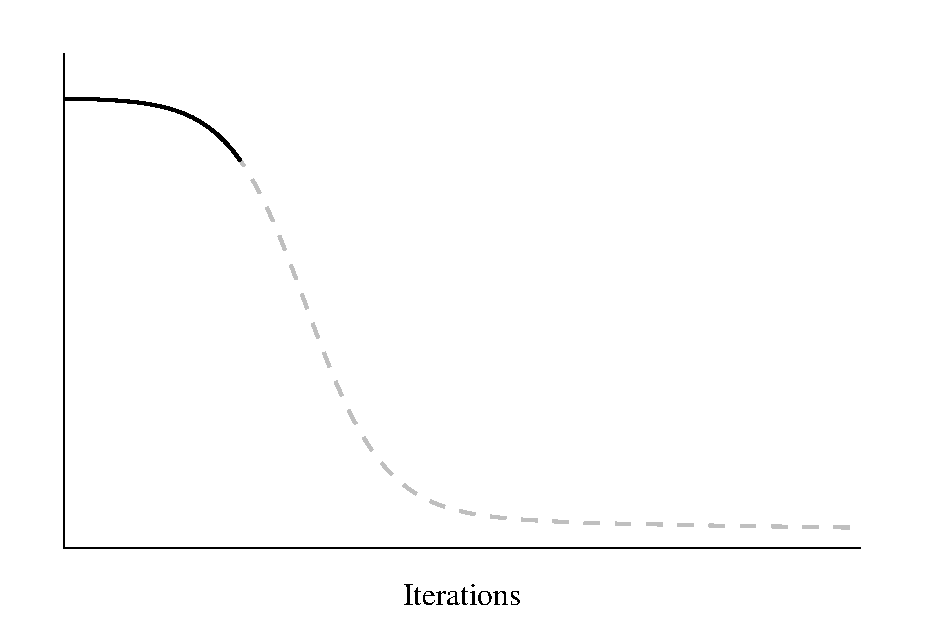
\includegraphics[width=5cm]{convergence1.eps}};
  \node[rotate=90] at (15.5,3) { $\left| \mathbb{E} \! \left[ f \right] - \hat{f} \right|$ };
\end{tikzpicture}
}
\subfigure[]{
\begin{tikzpicture}[scale=0.25, thick]
  \draw[-,color=white] (-12, 0) to (12, 0);
  
  \begin{scope}
  \clip (-12, -10) rectangle (12, 10);
  \foreach \i in {0, 0.05,..., 1} {
    \draw[line width={30 * \i}, opacity={exp(-8 * \i)}, dark] 
      (-10, 0) .. controls (-10, 15) and (-5, 5) .. (0, 5)
      .. controls (5, 5) and (10, 8) .. (10, 0)
      .. controls (10, -8) and (5, -3) .. (0, -3)
      .. controls (-5, -3) and (-10, -5) .. (-10, 0);
  }
  
  % Convergence
  
  %\fill[color=dark] (-11, -8) circle (7pt);  
  %\fill[color=light] (-11, -8) circle (5pt);
  
  \fill[color=dark] (-10, -6.5) circle (7pt);  
  \fill[color=light] (-10, -6.5) circle (5pt);
  
  \fill[color=dark] (-9, -6.75) circle (7pt);  
  \fill[color=light] (-9, -6.75) circle (5pt);
  
  \fill[color=dark] (-8.25, -5) circle (7pt);  
  \fill[color=light] (-8.25, -5) circle (5pt);
  
  \fill[color=dark] (-7.5, -4) circle (7pt);  
  \fill[color=light] (-7.5, -4) circle (5pt);
  
  \fill[color=dark] (-7, -3.5) circle (7pt);  
  \fill[color=light] (-7, -3.5) circle (5pt);
  
  \fill[color=dark] (-6.5, -3.6) circle (7pt);  
  \fill[color=light] (-6.5, -3.6) circle (5pt);  
  
  % Mixing
  
  \fill[color=dark] (-6, -3) circle (7pt);  
  \fill[color=light] (-6, -3) circle (5pt);
  
  %\fill[color=dark] (-5.5, -3.5) circle (7pt);  
  %\fill[color=light] (-5.5, -3.5) circle (5pt);
  
  %\fill[color=dark] (-5, -3.75) circle (7pt);  
  %\fill[color=light] (-5, -3.75) circle (5pt);
  
  \fill[color=dark] (-4.75, -3.25) circle (7pt);  
  \fill[color=light] (-4.75, -3.25) circle (5pt);
  
  %\fill[color=dark] (-5, -3.5) circle (7pt);  
  %\fill[color=light] (-5, -3.5) circle (5pt);  
  
  %\fill[color=dark] (-4, -3.8) circle (7pt);  
  %\fill[color=light] (-4, -3.8) circle (5pt);
  
  \fill[color=dark] (-3, -3.5) circle (7pt);  
  \fill[color=light] (-3, -3.5) circle (5pt);
  
  %\fill[color=dark] (-2.8, -3) circle (7pt);  
  %\fill[color=light] (-2.8, -3) circle (5pt);
  
  %\fill[color=dark] (-2.9, -3.3) circle (7pt);  
  %\fill[color=light] (-2.9, -3.3) circle (5pt);  
  
  \fill[color=dark] (-2, -3.5) circle (7pt);  
  \fill[color=light] (-2, -3.5) circle (5pt);
  
  %\fill[color=dark] (-1.25, -3) circle (7pt);  
  %\fill[color=light] (-1.25, -3) circle (5pt);
  
  %\fill[color=dark] (-0.5, -2.75) circle (7pt);  
  %\fill[color=light] (-0.5, -2.75) circle (5pt);
  
  \fill[color=dark] (-0.3, -3) circle (7pt);  
  \fill[color=light] (-0.3, -3) circle (5pt);  
  
  %\fill[color=dark] (0.1, -2.75) circle (7pt);  
  %\fill[color=light] (0.1, -2.75) circle (5pt);
  
  %\fill[color=dark] (0.15, -3.1) circle (7pt);  
  %\fill[color=light] (0.15, -3.1) circle (5pt);  
  
  \fill[color=dark] (0.4, -3.4) circle (7pt);  
  \fill[color=light] (0.4, -3.4) circle (5pt);
  
  %\fill[color=dark] (1.1, -3.25) circle (7pt);  
  %\fill[color=light] (1.1, -3.25) circle (5pt);
  
  %\fill[color=dark] (2.7, -3.45) circle (7pt);  
  %\fill[color=light] (2.7, -3.45) circle (5pt);
  
  \fill[color=dark] (2.9, -3.2) circle (7pt);  
  \fill[color=light] (2.9, -3.2) circle (5pt);
  
  %\fill[color=dark] (3.1, -3.7) circle (7pt);  
  %\fill[color=light] (3.1, -3.7) circle (5pt);
  
  %\fill[color=dark] (4.2, -3.9) circle (7pt);  
  %\fill[color=light] (4.2, -3.9) circle (5pt);
  
  \fill[color=dark] (4, -4.1) circle (7pt);  
  \fill[color=light] (4, -4.1) circle (5pt);
  
  %\fill[color=dark] (5, -4) circle (7pt);  
  %\fill[color=light] (5, -4) circle (5pt);
  
  %\fill[color=dark] (5.8, -4.3) circle (7pt);  
  %\fill[color=light] (5.8, -4.3) circle (5pt);
  
  \fill[color=dark] (6.5, -4.8) circle (7pt);  
  \fill[color=light] (6.5, -4.8) circle (5pt);
  
  %\fill[color=dark] (6.8, -4.5) circle (7pt);  
  %\fill[color=light] (6.8, -4.5) circle (5pt);
  
  %\fill[color=dark] (7, -4.6) circle (7pt);  
  %\fill[color=light] (7, -4.6) circle (5pt);
  
  \fill[color=dark] (6.8, -4.7) circle (7pt);  
  \fill[color=light] (6.8, -4.7) circle (5pt);
  
  %\fill[color=dark] (7.75, -4.2) circle (7pt);  
  %\fill[color=light] (7.75, -4.2) circle (5pt);
  
  %\fill[color=dark] (8.5, -4.25) circle (7pt);  
  %\fill[color=light] (8.5, -4.25) circle (5pt);
  
  \fill[color=dark] (8.6, -4.75) circle (7pt);  
  \fill[color=light] (8.6, -4.75) circle (5pt);
  
  %\fill[color=dark] (8.8, -4.5) circle (7pt);  
  %\fill[color=light] (8.8, -4.5) circle (5pt);
  
  %\fill[color=dark] (9.25, -3.5) circle (7pt);  
  %\fill[color=light] (9.25, -3.5) circle (5pt);
  
  \fill[color=dark] (9.65, -2.75) circle (7pt);  
  \fill[color=light] (9.65, -2.75) circle (5pt);
  
  %\fill[color=dark] (9.5, -2) circle (7pt);  
  %\fill[color=light] (9.5, -2) circle (5pt);

  %\fill[color=dark] (9.8, -3) circle (7pt);  
  %\fill[color=light] (9.8, -3) circle (5pt);
  
  \fill[color=dark] (9.85, -0.8) circle (7pt);  
  \fill[color=light] (9.85, -0.8) circle (5pt);
  
  %\fill[color=dark] (10.1, -0.4) circle (7pt);  
  %\fill[color=light] (10.1, -0.4) circle (5pt);

  %\fill[color=dark] (10.25, 0.3) circle (7pt);  
  %\fill[color=light] (10.25, 0.3) circle (5pt);
  
  \fill[color=dark] (10, 0.7) circle (7pt);  
  \fill[color=light] (10, 0.7) circle (5pt);
  
  %\fill[color=dark] (9.7, 0.9) circle (7pt);  
  %\fill[color=light] (9.7, 0.9) circle (5pt);
  
  %\fill[color=dark] (10.3, 1.4) circle (7pt);  
  %\fill[color=light] (10.3, 1.4) circle (5pt);
  
  \fill[color=dark] (9.8, 2.25) circle (7pt);  
  \fill[color=light] (9.8, 2.25) circle (5pt);
  
  %\fill[color=dark] (10, 2.5) circle (7pt);  
  %\fill[color=light] (10, 2.5) circle (5pt);
  
  %\fill[color=dark] (10, 3) circle (7pt);  
  %\fill[color=light] (10, 3) circle (5pt);
  
  \fill[color=dark] (9.6, 3.75) circle (7pt);  
  \fill[color=light] (9.6, 3.75) circle (5pt);
  
  %\fill[color=dark] (9.1, 4.4) circle (7pt);  
  %\fill[color=light] (9.1, 4.4) circle (5pt);
  
  %\fill[color=dark] (9.1, 4.1) circle (7pt);  
  %\fill[color=light] (9.1, 4.1) circle (5pt);
  
  \fill[color=dark] (8.5, 4.75) circle (7pt);  
  \fill[color=light] (8.5, 4.75) circle (5pt);
  
  %\fill[color=dark] (8.1, 5.75) circle (7pt);  
  %\fill[color=light] (8.1, 5.75) circle (5pt);
  
  %\fill[color=dark] (7.7, 5.2) circle (7pt);  
  %\fill[color=light] (7.7, 5.2) circle (5pt);
  
  \fill[color=dark] (7.3, 5.3) circle (7pt);  
  \fill[color=light] (7.3, 5.3) circle (5pt);
  
  %\fill[color=dark] (6.6, 5.8) circle (7pt);  
  %\fill[color=light] (6.6, 5.8) circle (5pt);
  
  %\fill[color=dark] (6, 6) circle (7pt);  
  %\fill[color=light] (6, 6) circle (5pt);
  
  \fill[color=dark] (5.25, 5.45) circle (7pt);  
  \fill[color=light] (5.25, 5.45) circle (5pt);
  
  %\fill[color=dark] (4.75, 5.75) circle (7pt);  
  %\fill[color=light] (4.75, 5.75) circle (5pt);
  
  %\fill[color=dark] (3.5, 5.28) circle (7pt);  
  %\fill[color=light] (3.5, 5.28) circle (5pt);
  
  \fill[color=dark] (5, 5.65) circle (7pt);  
  \fill[color=light] (5, 5.65) circle (5pt);
  
  %\fill[color=dark] (3, 5.5) circle (7pt);  
  %\fill[color=light] (3, 5.5) circle (5pt);
  
  %\fill[color=dark] (2.75, 5.3) circle (7pt);  
  %\fill[color=light] (2.75, 5.3) circle (5pt);
  
  \fill[color=dark] (2.25, 4.8) circle (7pt);  
  \fill[color=light] (2.25, 4.8) circle (5pt);
  
  %\fill[color=dark] (2, 5.2) circle (7pt);  
  %\fill[color=light] (2, 5.2) circle (5pt);
  
  %\fill[color=dark] (1.75, 4.9) circle (7pt);  
  %\fill[color=light] (1.75, 4.9) circle (5pt);
  
  \fill[color=dark] (1.5, 5.1) circle (7pt);  
  \fill[color=light] (1.5, 5.1) circle (5pt);
  
  %\fill[color=dark] (0.8, 5.2) circle (7pt);  
  %\fill[color=light] (0.8, 5.2) circle (5pt);
 
  %\fill[color=dark] (0, 4.7) circle (7pt);  
  %\fill[color=light] (0, 4.7) circle (5pt);
  
  \fill[color=dark] (-0.6, 5) circle (7pt);  
  \fill[color=light] (-0.6, 5) circle (5pt);
  
  %\fill[color=dark] (-1.25, 5.2) circle (7pt);  
  %\fill[color=light] (-1.25, 5.2) circle (5pt);
  
  %\fill[color=dark] (-1.55, 5.4) circle (7pt);  
  %\fill[color=light] (-1.55, 5.4) circle (5pt);
  
  \fill[color=dark] (-1.85, 5) circle (7pt);  
  \fill[color=light] (-1.85, 5) circle (5pt);
  
  %\fill[color=dark] (-2.75, 5.5) circle (7pt);  
  %\fill[color=light] (-2.75, 5.5) circle (5pt);
  
  %\fill[color=dark] (-3.5, 6.6) circle (7pt);  
  %\fill[color=light] (-3.5, 6.6) circle (5pt);
  
  \fill[color=dark] (-4.25, 6.5) circle (7pt);  
  \fill[color=light] (-4.25, 6.5) circle (5pt);
  
  %\fill[color=dark] (-4.9, 7.2) circle (7pt);  
  %\fill[color=light] (-4.9, 7.2) circle (5pt);
  
  %\fill[color=dark] (-5.2, 7) circle (7pt);  
  %\fill[color=light] (-5.2, 7) circle (5pt);
  
  \fill[color=dark] (-5.75, 7.4) circle (7pt);  
  \fill[color=light] (-5.75, 7.4) circle (5pt);
  
  %\fill[color=dark] (-6, 7.9) circle (7pt);  
  %\fill[color=light] (-6, 7.9) circle (5pt);
  
  %\fill[color=dark] (-6.25, 7.8) circle (7pt);  
  %\fill[color=light] (-6.25, 7.8) circle (5pt);
  
  \fill[color=dark] (-6.5, 7.5) circle (7pt);  
  \fill[color=light] (-6.5, 7.5) circle (5pt);
  
  %\fill[color=dark] (-6.75, 8) circle (7pt);  
  %\fill[color=light] (-6.75, 8) circle (5pt);
  
  %\fill[color=dark] (-7.5, 8.5) circle (7pt);  
  %\fill[color=light] (-7.5, 8.5) circle (5pt);
  
  \fill[color=dark] (-8.25, 8) circle (7pt);  
  \fill[color=light] (-8.25, 8) circle (5pt);
  
  %\fill[color=dark] (-8.65, 7.8) circle (7pt);  
  %\fill[color=light] (-8.65, 7.8) circle (5pt);
  
  %\fill[color=dark] (-8.4, 7.7) circle (7pt);  
  %\fill[color=light] (-8.4, 7.7) circle (5pt);
  
  \fill[color=dark] (-9.2, 7) circle (7pt);  
  \fill[color=light] (-9.2, 7) circle (5pt);
  
  %\fill[color=dark] (-9.5, 6.75) circle (7pt);  
  %\fill[color=light] (-9.5, 6.75) circle (5pt);
  
  %\fill[color=dark] (-10, 6) circle (7pt);  
  %\fill[color=light] (-10, 6) circle (5pt);
  
  \fill[color=dark] (-9.7, 5.3) circle (7pt);  
  \fill[color=light] (-9.7, 5.3) circle (5pt);
  
  %\fill[color=dark] (-9.6, 5) circle (7pt);  
  %\fill[color=light] (-9.6, 5) circle (5pt);
  
  %\fill[color=dark] (-9.9, 4.75) circle (7pt);  
  %\fill[color=light] (-9.9, 4.75) circle (5pt);
  
  \fill[color=dark] (-10.1, 4) circle (7pt);  
  \fill[color=light] (-10.1, 4) circle (5pt);
  
  %\fill[color=dark] (-9.7, 3.5) circle (7pt);  
  %\fill[color=light] (-9.7, 3.5) circle (5pt);
  
  %\fill[color=dark] (-9.8, 3) circle (7pt);  
  %\fill[color=light] (-9.8, 3) circle (5pt);
  
  \fill[color=dark] (-10, 2.2) circle (7pt);  
  \fill[color=light] (-10, 2.2) circle (5pt);  
  
  %\fill[color=dark] (-10.25, 1.9) circle (7pt);  
  %\fill[color=light] (-10.25, 1.9) circle (5pt);  
  
  %\fill[color=dark] (-9.7, 1.8) circle (7pt);  
  %\fill[color=light] (-9.7, 1.8) circle (5pt);  
  
  \fill[color=dark] (-10.2, 1.4) circle (7pt);  
  \fill[color=light] (-10.2, 1.4) circle (5pt);  
  
  %\fill[color=dark] (-9.8, 0.7) circle (7pt);  
  %\fill[color=light] (-9.8, 0.7) circle (5pt);  
  
  %\fill[color=dark] (-10.2, 0.1) circle (7pt);  
  %\fill[color=light] (-10.2, 0.1) circle (5pt);  
  
  \fill[color=dark] (-9.9, -0.1) circle (7pt);  
  \fill[color=light] (-9.9, -0.1) circle (5pt);  
  
  %\fill[color=dark] (-10, -0.9) circle (7pt);  
  %\fill[color=light] (-10, -0.9) circle (5pt);  
  
  %\fill[color=dark] (-9.6, -1.5) circle (7pt);  
  %\fill[color=light] (-9.6, -1.5) circle (5pt);  
  
  \fill[color=dark] (-9.5, -1.8) circle (7pt);  
  \fill[color=light] (-9.5, -1.8) circle (5pt);  
  
  %\fill[color=dark] (-9.7, -2.1) circle (7pt);  
  %\fill[color=light] (-9.7, -2.1) circle (5pt);  
  
  %\fill[color=dark] (-9.3, -2.8) circle (7pt);  
  %\fill[color=light] (-9.3, -2.8) circle (5pt);  
  
  \fill[color=dark] (-8.3, -3) circle (7pt);  
  \fill[color=light] (-8.3, -3) circle (5pt);  
  
  %\fill[color=dark] (-7.8, -3.4) circle (7pt);  
  %\fill[color=light] (-7.8, -3.4) circle (5pt);  
  
  %\fill[color=dark] (-7.6, -3) circle (7pt);  
  %\fill[color=light] (-7.6, -3) circle (5pt);   
  
  \end{scope}
  
  \draw[-,color=white] (14, 0) to (38, 0);  
  \node[] at (28,3) {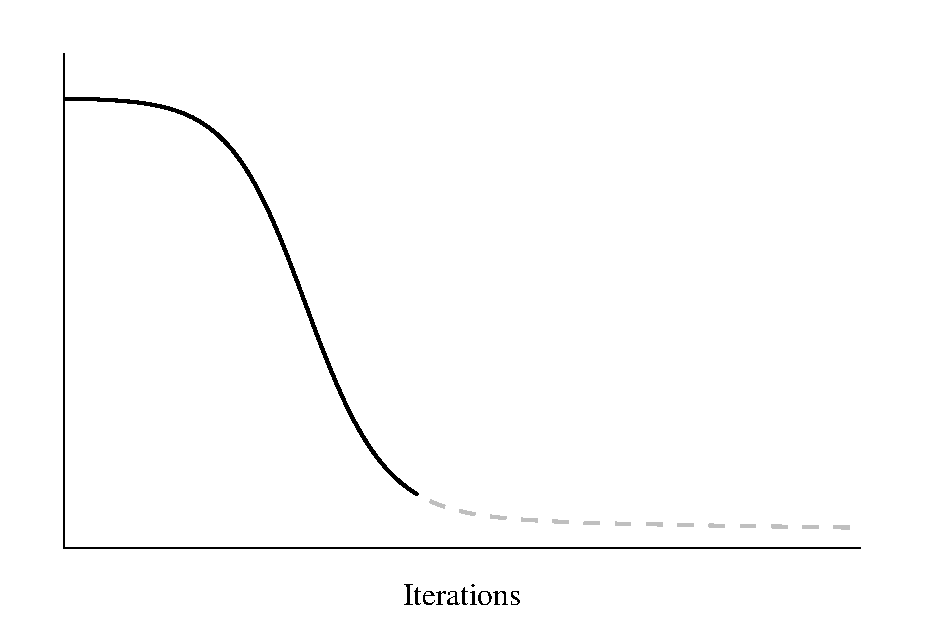
\includegraphics[width=5cm]{convergence2.eps}};
  \node[rotate=90] at (15.5,3) { $\left| \mathbb{E} \! \left[ f \right] - \hat{f} \right|$ };
\end{tikzpicture}
}
\subfigure[]{
\begin{tikzpicture}[scale=0.25, thick]
  \draw[-,color=white] (-12, 0) to (12, 0);
  
  \begin{scope}
  \clip (-12, -10) rectangle (12, 10);
  \foreach \i in {0, 0.05,..., 1} {
    \draw[line width={30 * \i}, opacity={exp(-8 * \i)}, dark] 
      (-10, 0) .. controls (-10, 15) and (-5, 5) .. (0, 5)
      .. controls (5, 5) and (10, 8) .. (10, 0)
      .. controls (10, -8) and (5, -3) .. (0, -3)
      .. controls (-5, -3) and (-10, -5) .. (-10, 0);
  }
  
  %\fill[color=dark] (-11, -8) circle (7pt);  
  %\fill[color=light] (-11, -8) circle (5pt);
  
  \fill[color=dark] (-10, -6.5) circle (7pt);  
  \fill[color=light] (-10, -6.5) circle (5pt);
  
  \fill[color=dark] (-9, -6.75) circle (7pt);  
  \fill[color=light] (-9, -6.75) circle (5pt);
  
  \fill[color=dark] (-8.25, -5) circle (7pt);  
  \fill[color=light] (-8.25, -5) circle (5pt);
  
  \fill[color=dark] (-7.5, -4) circle (7pt);  
  \fill[color=light] (-7.5, -4) circle (5pt);
  
  \fill[color=dark] (-7, -3.5) circle (7pt);  
  \fill[color=light] (-7, -3.5) circle (5pt);
  
  \fill[color=dark] (-6.5, -3.6) circle (7pt);  
  \fill[color=light] (-6.5, -3.6) circle (5pt);  
  
  \fill[color=dark] (-6, -3) circle (7pt);  
  \fill[color=light] (-6, -3) circle (5pt);
  
  \fill[color=dark] (-5.5, -3.5) circle (7pt);  
  \fill[color=light] (-5.5, -3.5) circle (5pt);
  
  \fill[color=dark] (-5, -3.75) circle (7pt);  
  \fill[color=light] (-5, -3.75) circle (5pt);
  
  \fill[color=dark] (-4.75, -3.25) circle (7pt);  
  \fill[color=light] (-4.75, -3.25) circle (5pt);
  
  \fill[color=dark] (-5, -3.5) circle (7pt);  
  \fill[color=light] (-5, -3.5) circle (5pt);  
  
  \fill[color=dark] (-4, -3.8) circle (7pt);  
  \fill[color=light] (-4, -3.8) circle (5pt);
  
  \fill[color=dark] (-3, -3.5) circle (7pt);  
  \fill[color=light] (-3, -3.5) circle (5pt);
  
  \fill[color=dark] (-2.8, -3) circle (7pt);  
  \fill[color=light] (-2.8, -3) circle (5pt);
  
  \fill[color=dark] (-2.9, -3.3) circle (7pt);  
  \fill[color=light] (-2.9, -3.3) circle (5pt);  
  
  \fill[color=dark] (-2, -3.5) circle (7pt);  
  \fill[color=light] (-2, -3.5) circle (5pt);
  
  \fill[color=dark] (-1.25, -3) circle (7pt);  
  \fill[color=light] (-1.25, -3) circle (5pt);
  
  \fill[color=dark] (-0.5, -2.75) circle (7pt);  
  \fill[color=light] (-0.5, -2.75) circle (5pt);
  
  \fill[color=dark] (-0.3, -3) circle (7pt);  
  \fill[color=light] (-0.3, -3) circle (5pt);  
  
  \fill[color=dark] (0.1, -2.75) circle (7pt);  
  \fill[color=light] (0.1, -2.75) circle (5pt);
  
  \fill[color=dark] (0.15, -3.1) circle (7pt);  
  \fill[color=light] (0.15, -3.1) circle (5pt);  
  
  \fill[color=dark] (0.4, -3.4) circle (7pt);  
  \fill[color=light] (0.4, -3.4) circle (5pt);
  
  \fill[color=dark] (1.1, -3.25) circle (7pt);  
  \fill[color=light] (1.1, -3.25) circle (5pt);
  
  \fill[color=dark] (2.7, -3.45) circle (7pt);  
  \fill[color=light] (2.7, -3.45) circle (5pt);
  
  \fill[color=dark] (2.9, -3.2) circle (7pt);  
  \fill[color=light] (2.9, -3.2) circle (5pt);
  
  \fill[color=dark] (3.1, -3.7) circle (7pt);  
  \fill[color=light] (3.1, -3.7) circle (5pt);
  
  \fill[color=dark] (4.2, -3.9) circle (7pt);  
  \fill[color=light] (4.2, -3.9) circle (5pt);
  
  \fill[color=dark] (4, -4.1) circle (7pt);  
  \fill[color=light] (4, -4.1) circle (5pt);
  
  \fill[color=dark] (5, -4) circle (7pt);  
  \fill[color=light] (5, -4) circle (5pt);
  
  \fill[color=dark] (5.8, -4.3) circle (7pt);  
  \fill[color=light] (5.8, -4.3) circle (5pt);
  
  \fill[color=dark] (6.5, -4.8) circle (7pt);  
  \fill[color=light] (6.5, -4.8) circle (5pt);
  
  \fill[color=dark] (6.8, -4.5) circle (7pt);  
  \fill[color=light] (6.8, -4.5) circle (5pt);
  
  \fill[color=dark] (7, -4.6) circle (7pt);  
  \fill[color=light] (7, -4.6) circle (5pt);
  
  \fill[color=dark] (6.8, -4.7) circle (7pt);  
  \fill[color=light] (6.8, -4.7) circle (5pt);
  
  \fill[color=dark] (7.75, -4.2) circle (7pt);  
  \fill[color=light] (7.75, -4.2) circle (5pt);
  
  \fill[color=dark] (8.5, -4.25) circle (7pt);  
  \fill[color=light] (8.5, -4.25) circle (5pt);
  
  \fill[color=dark] (8.6, -4.75) circle (7pt);  
  \fill[color=light] (8.6, -4.75) circle (5pt);
  
  \fill[color=dark] (8.8, -4.5) circle (7pt);  
  \fill[color=light] (8.8, -4.5) circle (5pt);
  
  \fill[color=dark] (9.25, -3.5) circle (7pt);  
  \fill[color=light] (9.25, -3.5) circle (5pt);
  
  \fill[color=dark] (9.65, -2.75) circle (7pt);  
  \fill[color=light] (9.65, -2.75) circle (5pt);
  
  \fill[color=dark] (9.5, -2) circle (7pt);  
  \fill[color=light] (9.5, -2) circle (5pt);

  \fill[color=dark] (9.8, -3) circle (7pt);  
  \fill[color=light] (9.8, -3) circle (5pt);
  
  \fill[color=dark] (9.85, -0.8) circle (7pt);  
  \fill[color=light] (9.85, -0.8) circle (5pt);
  
  \fill[color=dark] (10.1, -0.4) circle (7pt);  
  \fill[color=light] (10.1, -0.4) circle (5pt);

  \fill[color=dark] (10.25, 0.3) circle (7pt);  
  \fill[color=light] (10.25, 0.3) circle (5pt);
  
  \fill[color=dark] (10, 0.7) circle (7pt);  
  \fill[color=light] (10, 0.7) circle (5pt);
  
  \fill[color=dark] (9.7, 0.9) circle (7pt);  
  \fill[color=light] (9.7, 0.9) circle (5pt);
  
  \fill[color=dark] (10.3, 1.4) circle (7pt);  
  \fill[color=light] (10.3, 1.4) circle (5pt);
  
  \fill[color=dark] (9.8, 2.25) circle (7pt);  
  \fill[color=light] (9.8, 2.25) circle (5pt);
  
  \fill[color=dark] (10, 2.5) circle (7pt);  
  \fill[color=light] (10, 2.5) circle (5pt);
  
  \fill[color=dark] (10, 3) circle (7pt);  
  \fill[color=light] (10, 3) circle (5pt);
  
  \fill[color=dark] (9.6, 3.75) circle (7pt);  
  \fill[color=light] (9.6, 3.75) circle (5pt);
  
  \fill[color=dark] (9.1, 4.4) circle (7pt);  
  \fill[color=light] (9.1, 4.4) circle (5pt);
  
  \fill[color=dark] (9.1, 4.1) circle (7pt);  
  \fill[color=light] (9.1, 4.1) circle (5pt);
  
  \fill[color=dark] (8.5, 4.75) circle (7pt);  
  \fill[color=light] (8.5, 4.75) circle (5pt);
  
  \fill[color=dark] (8.1, 5.75) circle (7pt);  
  \fill[color=light] (8.1, 5.75) circle (5pt);
  
  \fill[color=dark] (7.7, 5.2) circle (7pt);  
  \fill[color=light] (7.7, 5.2) circle (5pt);
  
  \fill[color=dark] (7.3, 5.3) circle (7pt);  
  \fill[color=light] (7.3, 5.3) circle (5pt);
  
  \fill[color=dark] (6.6, 5.8) circle (7pt);  
  \fill[color=light] (6.6, 5.8) circle (5pt);
  
  \fill[color=dark] (6, 6) circle (7pt);  
  \fill[color=light] (6, 6) circle (5pt);
  
  \fill[color=dark] (5.25, 5.45) circle (7pt);  
  \fill[color=light] (5.25, 5.45) circle (5pt);
  
  \fill[color=dark] (4.75, 5.75) circle (7pt);  
  \fill[color=light] (4.75, 5.75) circle (5pt);
  
  \fill[color=dark] (3.5, 5.28) circle (7pt);  
  \fill[color=light] (3.5, 5.28) circle (5pt);
  
  \fill[color=dark] (5, 5.65) circle (7pt);  
  \fill[color=light] (5, 5.65) circle (5pt);
  
  \fill[color=dark] (3, 5.5) circle (7pt);  
  \fill[color=light] (3, 5.5) circle (5pt);
  
  \fill[color=dark] (2.75, 5.3) circle (7pt);  
  \fill[color=light] (2.75, 5.3) circle (5pt);
  
  \fill[color=dark] (2.25, 4.8) circle (7pt);  
  \fill[color=light] (2.25, 4.8) circle (5pt);
  
  \fill[color=dark] (2, 5.2) circle (7pt);  
  \fill[color=light] (2, 5.2) circle (5pt);
  
  \fill[color=dark] (1.75, 4.9) circle (7pt);  
  \fill[color=light] (1.75, 4.9) circle (5pt);
  
  \fill[color=dark] (1.5, 5.1) circle (7pt);  
  \fill[color=light] (1.5, 5.1) circle (5pt);
  
  \fill[color=dark] (0.8, 5.2) circle (7pt);  
  \fill[color=light] (0.8, 5.2) circle (5pt);
 
  \fill[color=dark] (0, 4.7) circle (7pt);  
  \fill[color=light] (0, 4.7) circle (5pt);
  
  \fill[color=dark] (-0.6, 5) circle (7pt);  
  \fill[color=light] (-0.6, 5) circle (5pt);
  
  \fill[color=dark] (-1.25, 5.2) circle (7pt);  
  \fill[color=light] (-1.25, 5.2) circle (5pt);
  
  \fill[color=dark] (-1.55, 5.4) circle (7pt);  
  \fill[color=light] (-1.55, 5.4) circle (5pt);
  
  \fill[color=dark] (-1.85, 5) circle (7pt);  
  \fill[color=light] (-1.85, 5) circle (5pt);
  
  \fill[color=dark] (-2.75, 5.5) circle (7pt);  
  \fill[color=light] (-2.75, 5.5) circle (5pt);
  
  \fill[color=dark] (-3.5, 6.6) circle (7pt);  
  \fill[color=light] (-3.5, 6.6) circle (5pt);
  
  \fill[color=dark] (-4.25, 6.5) circle (7pt);  
  \fill[color=light] (-4.25, 6.5) circle (5pt);
  
  \fill[color=dark] (-4.9, 7.2) circle (7pt);  
  \fill[color=light] (-4.9, 7.2) circle (5pt);
  
  \fill[color=dark] (-5.2, 7) circle (7pt);  
  \fill[color=light] (-5.2, 7) circle (5pt);
  
  \fill[color=dark] (-5.75, 7.4) circle (7pt);  
  \fill[color=light] (-5.75, 7.4) circle (5pt);
  
  \fill[color=dark] (-6, 7.9) circle (7pt);  
  \fill[color=light] (-6, 7.9) circle (5pt);
  
  \fill[color=dark] (-6.25, 7.8) circle (7pt);  
  \fill[color=light] (-6.25, 7.8) circle (5pt);
  
  \fill[color=dark] (-6.5, 7.5) circle (7pt);  
  \fill[color=light] (-6.5, 7.5) circle (5pt);
  
  \fill[color=dark] (-6.75, 8) circle (7pt);  
  \fill[color=light] (-6.75, 8) circle (5pt);
  
  \fill[color=dark] (-7.5, 8.5) circle (7pt);  
  \fill[color=light] (-7.5, 8.5) circle (5pt);
  
  \fill[color=dark] (-8.25, 8) circle (7pt);  
  \fill[color=light] (-8.25, 8) circle (5pt);
  
  \fill[color=dark] (-8.65, 7.8) circle (7pt);  
  \fill[color=light] (-8.65, 7.8) circle (5pt);
  
  \fill[color=dark] (-8.4, 7.7) circle (7pt);  
  \fill[color=light] (-8.4, 7.7) circle (5pt);
  
  \fill[color=dark] (-9.2, 7) circle (7pt);  
  \fill[color=light] (-9.2, 7) circle (5pt);
  
  \fill[color=dark] (-9.5, 6.75) circle (7pt);  
  \fill[color=light] (-9.5, 6.75) circle (5pt);
  
  \fill[color=dark] (-10, 6) circle (7pt);  
  \fill[color=light] (-10, 6) circle (5pt);
  
  \fill[color=dark] (-9.7, 5.3) circle (7pt);  
  \fill[color=light] (-9.7, 5.3) circle (5pt);
  
  \fill[color=dark] (-9.6, 5) circle (7pt);  
  \fill[color=light] (-9.6, 5) circle (5pt);
  
  \fill[color=dark] (-9.9, 4.75) circle (7pt);  
  \fill[color=light] (-9.9, 4.75) circle (5pt);
  
  \fill[color=dark] (-10.1, 4) circle (7pt);  
  \fill[color=light] (-10.1, 4) circle (5pt);
  
  \fill[color=dark] (-9.7, 3.5) circle (7pt);  
  \fill[color=light] (-9.7, 3.5) circle (5pt);
  
  \fill[color=dark] (-9.8, 3) circle (7pt);  
  \fill[color=light] (-9.8, 3) circle (5pt);
  
  \fill[color=dark] (-10, 2.2) circle (7pt);  
  \fill[color=light] (-10, 2.2) circle (5pt);  
  
  \fill[color=dark] (-10.25, 1.9) circle (7pt);  
  \fill[color=light] (-10.25, 1.9) circle (5pt);  
  
  \fill[color=dark] (-9.7, 1.8) circle (7pt);  
  \fill[color=light] (-9.7, 1.8) circle (5pt);  
  
  \fill[color=dark] (-10.2, 1.4) circle (7pt);  
  \fill[color=light] (-10.2, 1.4) circle (5pt);  
  
  \fill[color=dark] (-9.8, 0.7) circle (7pt);  
  \fill[color=light] (-9.8, 0.7) circle (5pt);  
  
  \fill[color=dark] (-10.2, 0.1) circle (7pt);  
  \fill[color=light] (-10.2, 0.1) circle (5pt);  
  
  \fill[color=dark] (-9.9, -0.1) circle (7pt);  
  \fill[color=light] (-9.9, -0.1) circle (5pt);  
  
  \fill[color=dark] (-10, -0.9) circle (7pt);  
  \fill[color=light] (-10, -0.9) circle (5pt);  
  
  \fill[color=dark] (-9.6, -1.5) circle (7pt);  
  \fill[color=light] (-9.6, -1.5) circle (5pt);  
  
  \fill[color=dark] (-9.5, -1.8) circle (7pt);  
  \fill[color=light] (-9.5, -1.8) circle (5pt);  
  
  \fill[color=dark] (-9.7, -2.1) circle (7pt);  
  \fill[color=light] (-9.7, -2.1) circle (5pt);  
  
  \fill[color=dark] (-9.3, -2.8) circle (7pt);  
  \fill[color=light] (-9.3, -2.8) circle (5pt);  
  
  \fill[color=dark] (-8.3, -3) circle (7pt);  
  \fill[color=light] (-8.3, -3) circle (5pt);  
  
  \fill[color=dark] (-7.8, -3.4) circle (7pt);  
  \fill[color=light] (-7.8, -3.4) circle (5pt);  
  
  \fill[color=dark] (-7.6, -3) circle (7pt);  
  \fill[color=light] (-7.6, -3) circle (5pt);   
  
  \end{scope}
  
  \draw[-,color=white] (14, 0) to (38, 0);  
  \node[] at (28,3) {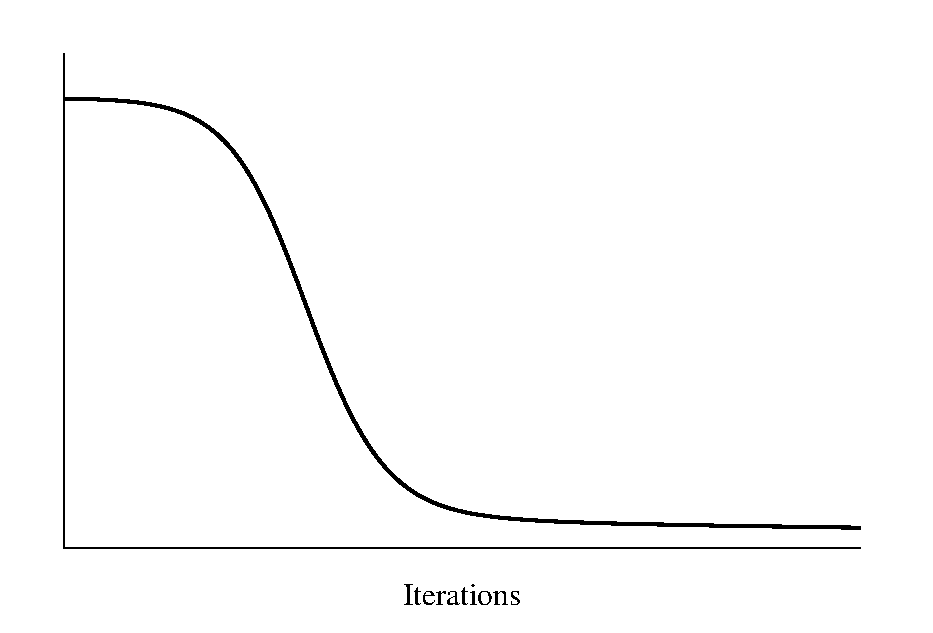
\includegraphics[width=5cm]{convergence3.eps}};
  \node[rotate=90] at (15.5,3) { $\left| \mathbb{E} \! \left[ f \right] - \hat{f} \right|$ };
\end{tikzpicture}
}
\caption{Under ideal circumstances, a Markov chain explores 
the target distribution in three phases.  (a) First the Markov
chain convergences to the typical set and estimators suffer
from initial but ultimately transient biases. (b) Once the Markov 
chain finds the typical set and makes it first sojourn through it,
this initial bias rapidly vanishes and the estimators become
much more accurate.  (c) As the Markov chain continues it
explores more details of the typical set and gradually improves
estimator precision.}
\label{fig:ideal_mcmc}
\end{figure*}

Once the Markov chain has entered into this third phase
the Markov chain Monte Carlo estimators satisfy a Central 
Limit Theorem
%
\begin{equation*}
\hat{f}_{N}^{\mathrm{MCMC}} \sim 
\mathcal{N} \! \left( \EE_{\PP} [ f ],
\mathrm{MCMCSE} \right),
\end{equation*}
%
where the \emph{Markov Chain Monte Carlo Standard Error} is 
given by
%
\begin{equation*}
\mathrm{MCMCSE} \equiv \sqrt{ \frac{ \mathrm{Var} [ f ] }{\mathrm{ESS} } }.
\end{equation*}
%
Here the \emph{effective sample size} is defined as
%
\begin{equation*}
\mathrm{ESS} = 
\frac{N}
{ 1 + 2 \sum_{l = 1}^{\infty} \rho_{l} },
\end{equation*}
%
where $\rho_{l}$ is the lag-$l$ autocorrelation of $f$ over the history
of the Markov chain.  As in the Importance Sampling Central Limit 
Theorem, the effective sample size quantifies the number of exact 
samples necessary to give an equivalent estimator precision and 
hence the effective number of exact samples ``contained'' in the 
Markov chain.  We can also interpret the effective sample size as 
the total number of sojourns the Markov chain has made through 
the typical set.

Because the states of the Markov chain during the initial convergence
phase mostly bias Markov chain Monte Carlo estimators, we can
achieve more precise estimators more quickly by using samples
generated only once the Markov chain has begun to explore the
typical set.  Consequently typical practice is to throw away some
number of initial samples before computing Markov chain Monte
Carlo estimators.

\subsubsection{Markov Chain Monte Carlo Under Less-Than-Ideal Conditions}

Under ideal conditions Markov chain Monte Carlo behaves
very similarly to Monte Carlo, only with a loss of efficiency due
to the correlation in the samples.  When the target distribution
exhibits more pathological behavior, however, Monte Carlo
continues to perform well while Markov chain Monte Carlo
begins to fail in spectacular fashion.

Consider, for example, a target probability distribution where
the typical set pinches into a region of high curvature
(Figure \ref{fig:pathological_typical_set}).  Most Markov
transitions do not have the resolution to maneuver into
these tight regions and the resulting Markov chains simply
ignore them, biasing subsequent Markov chain Monte Carlo
estimators.  It's as if there are thin but deep cracks hiding 
a significant amount of probability that the Markov chains 
pass right over and miss entirely.

\begin{figure*}
\centering
\begin{tikzpicture}[scale=0.3, thick]

\foreach \i in {0, 0.05,..., 1} {
  \begin{scope}
    \clip (-0.005, -9.5) rectangle (11, 6.5);
    \draw[line width={30 * \i}, opacity={exp(-8 * \i)}, dark] 
    (0, 5) .. controls (5, 5) and (10, 8) .. (10, 0)
             .. controls (10, -8) and (5, -3) .. (-2, -10);
  \end{scope}
  
  \begin{scope}
    \clip (0.005, -9.5) rectangle (-11, 6.5);
    \draw[line width={30 * \i}, opacity={exp(-8 * \i)}, dark] 
    (0, 5) .. controls (-5, 5) and (-10, 8) .. (-10, 0)
             .. controls (-10, -8) and (-5, -3) .. (2, -10);
  \end{scope}
}  
\fill[opacity=0.3, green] (0, -8.5) circle (1);
\end{tikzpicture}
%
\caption{Markov chains typically have trouble exploring regions 
of the typical set with large curvature (green), which induces
bias in Markov chain Monte Carlo estimators and spoils useful
behavior such as Central Limit Theorems.}
\label{fig:pathological_typical_set}
\end{figure*}

Because Markov chains have to recover the exact expectations
asymptotically, they have to somehow compensate for not being
able to explore these regions.  Typically the Markov chain
accomplishes this by getting stuck near the boundary of the
pathological region: as it hovers the estimators are drawn down 
as if the Markov chain were exploring the pathological region.
Eventually the Markov chain escapes to explore the rest of the
typical set and the estimator bias begins to increase again
(Figure \ref{fig:pathological exploration}).  

\begin{figure*}
\centering
\subfigure[]{
\begin{tikzpicture}[scale=0.25, thick]
  \draw[-,color=white] (-12, 0) to (12, 0);
  
  \foreach \i in {0, 0.05,..., 1} {
    \begin{scope}
      \clip (-0.005, -9.5) rectangle (11, 6.5);
      \draw[line width={30 * \i}, opacity={exp(-8 * \i)}, dark] 
      (0, 5) .. controls (5, 5) and (10, 8) .. (10, 0)
               .. controls (10, -8) and (5, -3) .. (-2, -10);
    \end{scope}
  
    \begin{scope}
      \clip (0.005, -9.5) rectangle (-11, 6.5);
      \draw[line width={30 * \i}, opacity={exp(-8 * \i)}, dark] 
      (0, 5) .. controls (-5, 5) and (-10, 8) .. (-10, 0)
               .. controls (-10, -8) and (-5, -3) .. (2, -10);
    \end{scope}
  }  
  \fill[opacity=0.3, green] (0, -8.5) circle (1);
  
  \fill[color=dark] (-8, 5.5) circle (7pt);  
  \fill[color=light] (-8, 5.5) circle (5pt);  
  
  \fill[color=dark] (-9, 4.75) circle (7pt);  
  \fill[color=light] (-9, 4.75) circle (5pt);  

  \fill[color=dark] (-8.7, 4.6) circle (7pt);  
  \fill[color=light] (-8.7, 4.6) circle (5pt); 
  
  \fill[color=dark] (-9.1, 4.5) circle (7pt);  
  \fill[color=light] (-9.1, 4.5) circle (5pt);  
  
  \fill[color=dark] (-9.2, 3.5) circle (7pt);  
  \fill[color=light] (-9.2, 3.5) circle (5pt);   
  
  \fill[color=dark] (-9.9, 3) circle (7pt);  
  \fill[color=light] (-9.9, 3) circle (5pt); 
  
  \fill[color=dark] (-10.1, 2.15) circle (7pt);  
  \fill[color=light] (-10.1, 2.15) circle (5pt);   
  
  \fill[color=dark] (-9.6, 1.5) circle (7pt);  
  \fill[color=light] (-9.6, 1.5) circle (5pt);   
  
  \fill[color=dark] (-9.75, 1) circle (7pt);  
  \fill[color=light] (-9.75, 1) circle (5pt); 
  
  \fill[color=dark] (-10.2, 0.25) circle (7pt);  
  \fill[color=light] (-10.2, 0.25) circle (5pt); 
  
  \fill[color=dark] (-9.8, 0) circle (7pt);  
  \fill[color=light] (-9.8, 0) circle (5pt); 
  
  \fill[color=dark] (-10, -0.5) circle (7pt);  
  \fill[color=light] (-10, -0.5) circle (5pt); 
  
  \fill[color=dark] (-9.75, -2) circle (7pt);  
  \fill[color=light] (-9.75, -2) circle (5pt);
  
  \fill[color=dark] (-9.9, -3) circle (7pt);  
  \fill[color=light] (-9.9, -3) circle (5pt);  
  
  \fill[color=dark] (-9.25, -3.5) circle (7pt);  
  \fill[color=light] (-9.25, -3.5) circle (5pt);   
  
  \fill[color=dark] (-9, -4.25) circle (7pt);  
  \fill[color=light] (-9, -4.25) circle (5pt);   
     
  \fill[color=dark] (-8, -4.5) circle (7pt);  
  \fill[color=light] (-8, -4.5) circle (5pt);  
  
  \fill[color=dark] (-8.25, -4.75) circle (7pt);  
  \fill[color=light] (-8.25, -4.75) circle (5pt);  

  \fill[color=dark] (-7.75, -5) circle (7pt);  
  \fill[color=light] (-7.75, -5) circle (5pt);  
  
  \fill[color=dark] (-6.5, -5.5) circle (7pt);  
  \fill[color=light] (-6.5, -5.5) circle (5pt);  
  
  \fill[color=dark] (-5.75, -5.25) circle (7pt);  
  \fill[color=light] (-5.75, -5.25) circle (5pt);  
  
  \fill[color=dark] (-5, -6) circle (7pt);  
  \fill[color=light] (-5, -6) circle (5pt);  
  
  \fill[color=dark] (-4.75, -6.25) circle (7pt);  
  \fill[color=light] (-4.75, -6.25) circle (5pt);  
  
  \fill[color=dark] (-3.8, -6) circle (7pt);  
  \fill[color=light] (-3.8, -6) circle (5pt);  
  
  \fill[color=dark] (-3.25, -6.5) circle (7pt);  
  \fill[color=light] (-3.25, -6.5) circle (5pt); 
  
  \fill[color=dark] (-2.75, -6.75) circle (7pt);  
  \fill[color=light] (-2.75, -6.75) circle (5pt);   
  
  \fill[color=dark] (-2, -7.5) circle (7pt);  
  \fill[color=light] (-2, -7.5) circle (5pt); 
  
  \fill[color=dark] (-1.75, -6.8) circle (7pt);  
  \fill[color=light] (-1.75, -6.8) circle (5pt);  
  
  \fill[color=dark] (-1.5, -7.2) circle (7pt);  
  \fill[color=light] (-1.5, -7.2) circle (5pt); 

  \draw[-,color=white] (14, 0) to (38, 0);  
  \node[] at (28,-2) {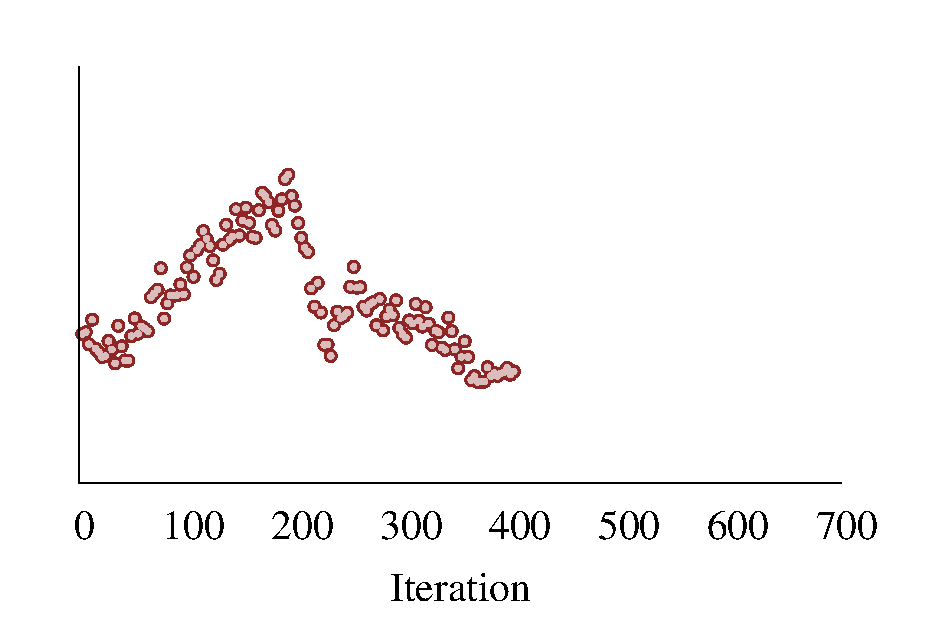
\includegraphics[width=6cm]{funnel_trace1.eps}};
\end{tikzpicture}
}
\subfigure[]{
\begin{tikzpicture}[scale=0.25, thick]
  \draw[-,color=white] (-12, 0) to (12, 0);
  
  \foreach \i in {0, 0.05,..., 1} {
    \begin{scope}
      \clip (-0.005, -9.5) rectangle (11, 6.5);
      \draw[line width={30 * \i}, opacity={exp(-8 * \i)}, dark] 
      (0, 5) .. controls (5, 5) and (10, 8) .. (10, 0)
               .. controls (10, -8) and (5, -3) .. (-2, -10);
    \end{scope}
  
    \begin{scope}
      \clip (0.005, -9.5) rectangle (-11, 6.5);
      \draw[line width={30 * \i}, opacity={exp(-8 * \i)}, dark] 
      (0, 5) .. controls (-5, 5) and (-10, 8) .. (-10, 0)
               .. controls (-10, -8) and (-5, -3) .. (2, -10);
    \end{scope}
  }  
  \fill[opacity=0.3, green] (0, -8.5) circle (1);
  
  \fill[color=dark] (-8, 5.5) circle (7pt);  
  \fill[color=light] (-8, 5.5) circle (5pt);  
  
  \fill[color=dark] (-9, 4.75) circle (7pt);  
  \fill[color=light] (-9, 4.75) circle (5pt);  

  \fill[color=dark] (-8.7, 4.6) circle (7pt);  
  \fill[color=light] (-8.7, 4.6) circle (5pt); 
  
  \fill[color=dark] (-9.1, 4.5) circle (7pt);  
  \fill[color=light] (-9.1, 4.5) circle (5pt);  
  
  \fill[color=dark] (-9.2, 3.5) circle (7pt);  
  \fill[color=light] (-9.2, 3.5) circle (5pt);   
  
  \fill[color=dark] (-9.9, 3) circle (7pt);  
  \fill[color=light] (-9.9, 3) circle (5pt); 
  
  \fill[color=dark] (-10.1, 2.15) circle (7pt);  
  \fill[color=light] (-10.1, 2.15) circle (5pt);   
  
  \fill[color=dark] (-9.6, 1.5) circle (7pt);  
  \fill[color=light] (-9.6, 1.5) circle (5pt);   
  
  \fill[color=dark] (-9.75, 1) circle (7pt);  
  \fill[color=light] (-9.75, 1) circle (5pt); 
  
  \fill[color=dark] (-10.2, 0.25) circle (7pt);  
  \fill[color=light] (-10.2, 0.25) circle (5pt); 
  
  \fill[color=dark] (-9.8, 0) circle (7pt);  
  \fill[color=light] (-9.8, 0) circle (5pt); 
  
  \fill[color=dark] (-10, -0.5) circle (7pt);  
  \fill[color=light] (-10, -0.5) circle (5pt); 
  
  \fill[color=dark] (-9.75, -2) circle (7pt);  
  \fill[color=light] (-9.75, -2) circle (5pt);
  
  \fill[color=dark] (-9.9, -3) circle (7pt);  
  \fill[color=light] (-9.9, -3) circle (5pt);  
  
  \fill[color=dark] (-9.25, -3.5) circle (7pt);  
  \fill[color=light] (-9.25, -3.5) circle (5pt);   
  
  \fill[color=dark] (-9, -4.25) circle (7pt);  
  \fill[color=light] (-9, -4.25) circle (5pt);   
     
  \fill[color=dark] (-8, -4.5) circle (7pt);  
  \fill[color=light] (-8, -4.5) circle (5pt);  
  
  \fill[color=dark] (-8.25, -4.75) circle (7pt);  
  \fill[color=light] (-8.25, -4.75) circle (5pt);  

  \fill[color=dark] (-7.75, -5) circle (7pt);  
  \fill[color=light] (-7.75, -5) circle (5pt);  
  
  \fill[color=dark] (-6.5, -5.5) circle (7pt);  
  \fill[color=light] (-6.5, -5.5) circle (5pt);  
  
  \fill[color=dark] (-5.75, -5.25) circle (7pt);  
  \fill[color=light] (-5.75, -5.25) circle (5pt);  
  
  \fill[color=dark] (-5, -6) circle (7pt);  
  \fill[color=light] (-5, -6) circle (5pt);  
  
  \fill[color=dark] (-4.75, -6.25) circle (7pt);  
  \fill[color=light] (-4.75, -6.25) circle (5pt);  
  
  \fill[color=dark] (-3.8, -6) circle (7pt);  
  \fill[color=light] (-3.8, -6) circle (5pt);  
  
  \fill[color=dark] (-3.25, -6.5) circle (7pt);  
  \fill[color=light] (-3.25, -6.5) circle (5pt); 
  
  \fill[color=dark] (-2.75, -6.75) circle (7pt);  
  \fill[color=light] (-2.75, -6.75) circle (5pt);   
  
  \fill[color=dark] (-2, -7.5) circle (7pt);  
  \fill[color=light] (-2, -7.5) circle (5pt); 
  
  \fill[color=dark] (-1.75, -6.8) circle (7pt);  
  \fill[color=light] (-1.75, -6.8) circle (5pt);  
  
  \fill[color=dark] (-1.5, -7.2) circle (7pt);  
  \fill[color=light] (-1.5, -7.2) circle (5pt); 
  
  \fill[color=dark] (-0.5, -7.5) circle (7pt);  
  \fill[color=light] (-0.5, -7.5) circle (5pt);
  
  \fill[color=dark] (0, -7.6) circle (7pt);  
  \fill[color=light] (0, -7.6) circle (5pt);  
  
  \fill[color=dark] (1, -7.7) circle (7pt);  
  \fill[color=light] (1, -7.7) circle (5pt);  

  \draw[-,color=white] (14, 0) to (38, 0);  
  \node[] at (28,-2) {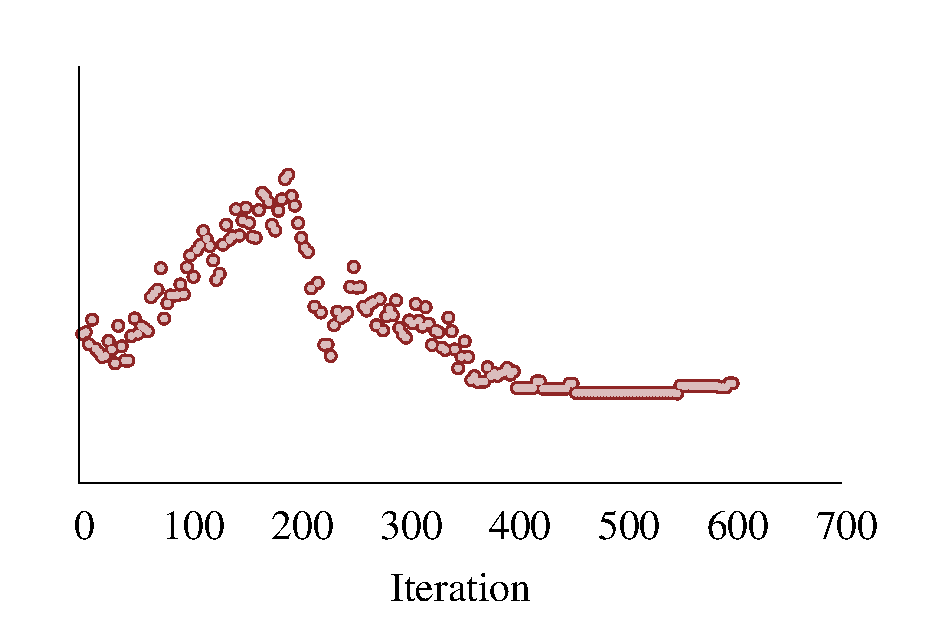
\includegraphics[width=6cm]{funnel_trace2.eps}};
\end{tikzpicture}
}
\subfigure[]{
\begin{tikzpicture}[scale=0.25, thick]
  \draw[-,color=white] (-12, 0) to (12, 0);
  
  \foreach \i in {0, 0.05,..., 1} {
    \begin{scope}
      \clip (-0.005, -9.5) rectangle (11, 6.5);
      \draw[line width={30 * \i}, opacity={exp(-8 * \i)}, dark] 
      (0, 5) .. controls (5, 5) and (10, 8) .. (10, 0)
               .. controls (10, -8) and (5, -3) .. (-2, -10);
    \end{scope}
  
    \begin{scope}
      \clip (0.005, -9.5) rectangle (-11, 6.5);
      \draw[line width={30 * \i}, opacity={exp(-8 * \i)}, dark] 
      (0, 5) .. controls (-5, 5) and (-10, 8) .. (-10, 0)
               .. controls (-10, -8) and (-5, -3) .. (2, -10);
    \end{scope}
  }  
  \fill[opacity=0.3, green] (0, -8.5) circle (1);
  
  \fill[color=dark] (-8, 5.5) circle (7pt);  
  \fill[color=light] (-8, 5.5) circle (5pt);  
  
  \fill[color=dark] (-9, 4.75) circle (7pt);  
  \fill[color=light] (-9, 4.75) circle (5pt);  

  \fill[color=dark] (-8.7, 4.6) circle (7pt);  
  \fill[color=light] (-8.7, 4.6) circle (5pt); 
  
  \fill[color=dark] (-9.1, 4.5) circle (7pt);  
  \fill[color=light] (-9.1, 4.5) circle (5pt);  
  
  \fill[color=dark] (-9.2, 3.5) circle (7pt);  
  \fill[color=light] (-9.2, 3.5) circle (5pt);   
  
  \fill[color=dark] (-9.9, 3) circle (7pt);  
  \fill[color=light] (-9.9, 3) circle (5pt); 
  
  \fill[color=dark] (-10.1, 2.15) circle (7pt);  
  \fill[color=light] (-10.1, 2.15) circle (5pt);   
  
  \fill[color=dark] (-9.6, 1.5) circle (7pt);  
  \fill[color=light] (-9.6, 1.5) circle (5pt);   
  
  \fill[color=dark] (-9.75, 1) circle (7pt);  
  \fill[color=light] (-9.75, 1) circle (5pt); 
  
  \fill[color=dark] (-10.2, 0.25) circle (7pt);  
  \fill[color=light] (-10.2, 0.25) circle (5pt); 
  
  \fill[color=dark] (-9.8, 0) circle (7pt);  
  \fill[color=light] (-9.8, 0) circle (5pt); 
  
  \fill[color=dark] (-10, -0.5) circle (7pt);  
  \fill[color=light] (-10, -0.5) circle (5pt); 
  
  \fill[color=dark] (-9.75, -2) circle (7pt);  
  \fill[color=light] (-9.75, -2) circle (5pt);
  
  \fill[color=dark] (-9.9, -3) circle (7pt);  
  \fill[color=light] (-9.9, -3) circle (5pt);  
  
  \fill[color=dark] (-9.25, -3.5) circle (7pt);  
  \fill[color=light] (-9.25, -3.5) circle (5pt);   
  
  \fill[color=dark] (-9, -4.25) circle (7pt);  
  \fill[color=light] (-9, -4.25) circle (5pt);   
     
  \fill[color=dark] (-8, -4.5) circle (7pt);  
  \fill[color=light] (-8, -4.5) circle (5pt);  
  
  \fill[color=dark] (-8.25, -4.75) circle (7pt);  
  \fill[color=light] (-8.25, -4.75) circle (5pt);  

  \fill[color=dark] (-7.75, -5) circle (7pt);  
  \fill[color=light] (-7.75, -5) circle (5pt);  
  
  \fill[color=dark] (-6.5, -5.5) circle (7pt);  
  \fill[color=light] (-6.5, -5.5) circle (5pt);  
  
  \fill[color=dark] (-5.75, -5.25) circle (7pt);  
  \fill[color=light] (-5.75, -5.25) circle (5pt);  
  
  \fill[color=dark] (-5, -6) circle (7pt);  
  \fill[color=light] (-5, -6) circle (5pt);  
  
  \fill[color=dark] (-4.75, -6.25) circle (7pt);  
  \fill[color=light] (-4.75, -6.25) circle (5pt);  
  
  \fill[color=dark] (-3.8, -6) circle (7pt);  
  \fill[color=light] (-3.8, -6) circle (5pt);  
  
  \fill[color=dark] (-3.25, -6.5) circle (7pt);  
  \fill[color=light] (-3.25, -6.5) circle (5pt); 
  
  \fill[color=dark] (-2.75, -6.75) circle (7pt);  
  \fill[color=light] (-2.75, -6.75) circle (5pt);   
  
  \fill[color=dark] (-2, -7.5) circle (7pt);  
  \fill[color=light] (-2, -7.5) circle (5pt); 
  
  \fill[color=dark] (-1.75, -6.8) circle (7pt);  
  \fill[color=light] (-1.75, -6.8) circle (5pt);  
  
  \fill[color=dark] (-1.5, -7.2) circle (7pt);  
  \fill[color=light] (-1.5, -7.2) circle (5pt); 
    
  \fill[color=dark] (-0.5, -7.5) circle (7pt);  
  \fill[color=light] (-0.5, -7.5) circle (5pt);
  
  \fill[color=dark] (0, -7.6) circle (7pt);  
  \fill[color=light] (0, -7.6) circle (5pt);  
  
  \fill[color=dark] (1, -7.7) circle (7pt);  
  \fill[color=light] (1, -7.7) circle (5pt);  
  
  \fill[color=dark] (9, 4.7) circle (7pt);  
  \fill[color=light] (9, 4.7) circle (5pt);  
  
  \fill[color=dark] (9.1, 4.25) circle (7pt);  
  \fill[color=light] (9.1, 4.25) circle (5pt);   
  
  \fill[color=dark] (9.8, 3) circle (7pt);  
  \fill[color=light] (9.8, 3) circle (5pt);   
  
  \fill[color=dark] (9.9, 1.5) circle (7pt);  
  \fill[color=light] (9.9, 1.5) circle (5pt);   
  
  \fill[color=dark] (9.75, -0.5) circle (7pt);  
  \fill[color=light] (9.75, -0.5) circle (5pt); 
  
  \fill[color=dark] (9.9, -1) circle (7pt);  
  \fill[color=light] (9.9, -1) circle (5pt);
  
  \fill[color=dark] (9.6, -3.5) circle (7pt);  
  \fill[color=light] (9.6, -3.5) circle (5pt);   
     
  \fill[color=dark] (7.8, -4.5) circle (7pt);  
  \fill[color=light] (7.8, -4.5) circle (5pt);  
  
  \fill[color=dark] (7, -5) circle (7pt);  
  \fill[color=light] (7, -5) circle (5pt);  
  
  \fill[color=dark] (6.5, -5.5) circle (7pt);  
  \fill[color=light] (6.5, -5.5) circle (5pt);  
  
  \fill[color=dark] (4.25, -6.5) circle (7pt);  
  \fill[color=light] (4.25, -6.5) circle (5pt);  
  
  \fill[color=dark] (2.1, -6.5) circle (7pt);  
  \fill[color=light] (2.1, -6.5) circle (5pt);   
  
  \draw[-,color=white] (14, 0) to (38, 0);  
  \node[] at (28,-2) {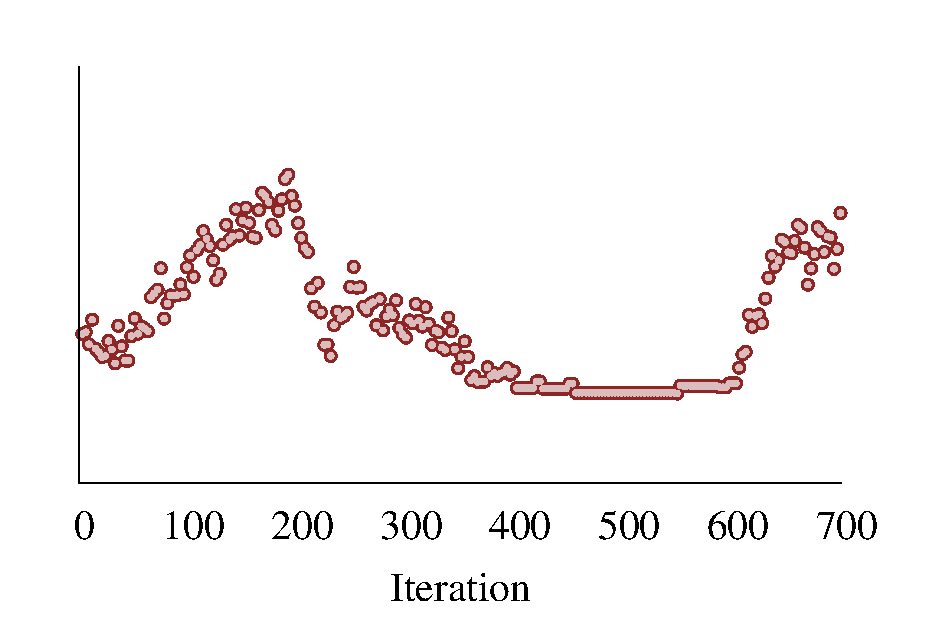
\includegraphics[width=6cm]{funnel_trace3.eps}};
\end{tikzpicture}
}
\caption{In practice, pathological regions of the typical set usually
cause Markov chains to get ``stuck''.  (a) Initially the Markov chain 
explores well-behaved regions of the typical set, avoiding the 
pathological neighborhood entirely and biasing Markov chain
Monte Carlo estimators.  (b) If the Markov chain is run long enough
then it will get stuck near the boundary of the pathological region, 
slowly correcting the Markov chain Monte Carlo estimators.  (c) 
Eventually the Markov chain escapes and explores the rest of 
the typical set.  This process repeats, causing the resulting 
estimators to oscillate around the true expectations in an unstable 
fashion.}
\label{fig:pathological exploration}
\end{figure*}

Ultimately this behavior results in estimators that oscillate 
around the true expectations.  Asymptotically the oscillations
average out to the true values, but that balance is delicate and
any finite time estimator will suffer from substantial biases.

Whether or not features of the target distribution become
pathological depends on how the Markov transition kernel
interacts with the target distribution.  Some transition kernels
are more robust than others and some can achieve robust
performance with careful tuning of auxiliary kernel parameters.
 
\subsubsection{MCMC in Practice}

In order to guarantee that we will not suffer from pathological
behavior we have to demonstrate strong \emph{ergodicity}
conditions that ensure the Markov chain not only explores
the typical set but does so sufficiently fast without being
hampered by pathological neighborhoods.  In most cases
we need to establish \emph{geometric ergodicity}.

Although we can identify generic features that often prevent
geometric ergodicity, determining whether or not a particular
Markov chain will exhibit pathological behavior when 
targeting a particular distribution is almost always infeasible
for nontrivial problems.  Moreover, there are no sufficient
conditions that we can use to establish geometric ergodicity
empirically.  Instead we have to rely on necessary conditions 
to provide any evidence that we can trust the resulting Markov 
chain Monte Carlo estimators.

Consequently we have to take great care when implementing
Markov chain Monte Carlo, and to maximize robust performance
we proceed in three stages.

\vspace{2mm}
\noindent \emph{Warmup}
\vspace{2mm}

We begin with \emph{warmup}, where we initialize multiple
chains from multiple, ideally diffuse, points in the sample space
and run long enough for them to converge to the typical set.
Because we do not include these warmup samples in any
Markov chain Monte Carlo estimators, we can also use this
period to adaptively tune any parameters in the Markov 
kernel without biasing our estimates.

Historically this stage has usually been called \emph{burn-in},
but we find that terminology inappropriate for Markov chain
Monte Carlo.  The problem is that burn-in is a process of 
stress-testing a system to identify and replace any failing
components.  In Markov chain Monte Carlo, however, any
misbehaving chains identify pathological behavior that is
biasing all of the chains and should very much not be ignored!
Because of this potentially-confusing, false analogy we use the
term warmup.

\vspace{2mm}
\noindent \emph{Sampling}
\vspace{2mm}

Once warmup as finished we begin a sampling phase where
we run the Markov chain and save all of the resulting samples
to construct Markov chain Monte Carlo estimators.

\vspace{2mm}
\noindent \emph{Evaluation}
\vspace{2mm}

Once both warmup and sampling have completed we can
search for any signs of pathological behavior and, if we
can't find any, move on to computing any desired estimator.

For what kind of pathological behavior should we be looking?
If we don't run warmup long enough for all of the Markov
chains to converge then not all of the Markov chains will look 
the same.  Similarly, any pathological regions in the typical set 
will bias the Markov chains in different ways.  Consequently a 
necessary condition for robust Markov chain Monte Carlo 
estimators is that each Markov chain appears identical.  In theory
we can quantify the homogeneity of our ensemble of Markov chains 
with the \emph{potential scale reduction factor} and in practice we
can estimate the potential scale reduction factor with the $\hat{R}$
statistic.

In addition to $\hat{R}$, specific Markov transitions may admit
their own, unique diagnostics sensitive to various pathologies
that can frustrate geometric ergodicity.

If we are confident that our Markov chains are exploring without
obstruction then we can finally compute Markov chain Monte
Carlo estimators using the samples generated in the sampling
phase.  If we also estimate the variances and autocorrelations
of each function then we can also quantify the error of these
estimates using an estimate of the Markov chain Monte Carlo
Standard Error.
